%%「論文」,「レター」,「レター(C分冊)」,「技術研究報告」などのテンプレート
%% 1. 「論文」
%% v1.6 [2009/11/03]
\documentclass[technicalreport]{ieicej}
%\documentclass[invited]{ieicej} % 招待論文
%\documentclass[comment]{ieicej} % 解説論文
\usepackage[dvipdfmx]{graphicx}
\usepackage{mediabb}
\usepackage{subfigure}
\usepackage{float}
\usepackage{latexsym}
\usepackage{url}
\usepackage[fleqn]{amsmath}
\usepackage[psamsfonts]{amssymb}

\setlength\intextsep{10pt}
\setlength\textfloatsep{0pt}

\setcounter{page}{1}

\field{A}
\jtitle{MultiPath TCP適用時のデータセンターネットワークでのフローサイズが与える影響に関する一考察}
\etitle{A study of the effect of the size of data flows in the data center network with MultiPath TCP}
\authorlist{%
 \authorentry{藤居 翔吾}{Shogo Fujii}{Hongo}% <= 記述しないとエラーになります
 \authorentry{田崎 創}{Hajime Tazaki}{IT}
 \authorentry{関谷 勇司}{Yuji Sekiya}{IT}
 %\authorentry{和文著者名}{英文著者名}{所属ラベル}
 %\authorentry[メールアドレス]{和文著者名}{英文著者名}{所属ラベル}
 %\authorentry{和文著者名}{英文著者名}{所属ラベル}[現在の所属ラベル]
}
\affiliate[Hongo]{東京大学大学院工学系研究科, 〒113-8656
東京都文京区本郷 7-3-1}{Graduate School of Engineering, 2-11-16 Hongo, Bunkyo-ku, Tokyo,
113-8656 Japan} \affiliate[IT]{東京大学情報基盤センター, 〒113-8658 東京都文京区弥生2-11-16}{The University of Tokyo, Information Technology Center, 2-11-16 Yayoi,
 Bunkyo-ku, Tokyo, 113-8658 Japan}
%\affiliate[所属ラベル]{和文所属}{英文所属}
%\paffiliate[]{}
%\paffiliate[現在の所属ラベル]{和文所属}

\begin{document}
\begin{abstract}
%和文あらまし 500字以内
データセンター内で運用されるサーバ台数の増加に伴い, それらを効率良く利用するためのネットワークトポロジーが研究されてきた.
近年では, Multipath TCP~(MPTCP) を用いて, さらなるネットワーク資源の有効活用を目指す取り組みが行われている.
また, 大規模データの分散処理技術により, ビッグデータを高速に処理することが可能になった.
近年の分散処理システムは, 管理ノードから発行されるQueryを処理ノードが実行するpartition-aggreateになっており,
データセンター内のネットワークにフローサイズの小さいトラフィックが大量に発生する.
MPTCPは複数の経路を同時に利用し, ネットワーク資源の有効活用を実現するが,
フローサイズの小さいトラフィックに関しては,
TCPよりも処理の完結に時間がかかり, その有用性に問題を抱えていると報告されている.
そこで本論文では、MPTCPを用いたデータセンターネットワークの有用性を検証し, Multipath
TCPのフローサイズが与える影響を考察する.
\end{abstract}
\begin{keyword}
%和文キーワード 4〜5語
MultiPath TCP, Short Flow, フロー完結時間, FatTree Topology, Datacenter network
\end{keyword}
\begin{eabstract}
As increasing the number of servers in a datacenter, the effective network
topology for utilization of massive computer clusters has been studied.
Recently, using MPTCP for the beneficial use has been tackled this problem.
As another solution, distributed processing system enabled to handle big data.
Today's the technique of distributed processing is that massive workers process data followed by the query from the master nodes.
As the result, a large quantity of short flow is generated in a datacenter network.
MPTCP can achieve the effective consumptions of the resources with multipath,
but a researcher reported MPTCP causes the delay of flow completion for short flows.
In this paper, we verified the utility of the datacenter network with MPTCP, and consider the effects of MPTCP by flow size.
%英文アブストラクト 100 words
\end{eabstract}
\begin{ekeyword}
Multipath TCP, Short flow, Flow completion time, FatTree topology, Datacenter
network
%英文キーワード
\end{ekeyword}
\maketitle

\section{まえがき}
\label{sec:intro}

多様な端末がネットワークに接続できるようになり, 様々な端末から大量かつ多種多様なデータの取得が可能となった.
特にデータ量の増加傾向は顕著で, 18$\sim$24ヶ月単位で総データ容量が2倍になるという予測がされている~\cite{IBM_rep}.
またFacebookでは, 300ペタバイト以上のデータ量を保有しており, 1日あたりに1ペタバイトのデータを解析している~\cite{presto}.
このように近年では, クラウドによるビッグデータの活用が着目され, ウェブ検索, SNSなど,
リアルタイムに近いレスポンスを返すような場面において使われ始めている.
そのようなクラウドサービスには近年要求が高まってきており, Amazonでは100[ms]の遅延により売り上げが1\%下がる,
といった報告~\cite{amazon}があるように, 遅延の影響は深刻な問題となっている.
そのため, 大規模データをより高速に解析することが求められており, データセンターでは,
コンピュータの運用台数が増加の一途をたどっている.
しかし, 大量の計算機資源から最大限の性能を引き出すためには, 従来の仕組みではデータセンター内トラフィックに対する不十分な帯域の割当により対応できないため,
計算機資源を有効活用するための研究が盛んに行われている.
そのようなスケーラビリティ拡大には, ネットワークトポロジー, アプリケーション, プロトコルに対するアプローチがある.

ネットワークトポロジーを改良するアプローチでは, 従来の単純な階層構造では,
データセンター内で発生するトラフィックに対して帯域が最大限割り当てられない~\cite{fattree}.
そのため, 近年ではそのようなトラフィックに対して帯域を有効利用するトポロジーが提案されている.

大量のデータの処理速度を改良するアプローチでは,
大量データ分散処理のためにpartition-aggregate計算モデルが提案されている.
MapReduce~\cite{mapreduce}, Dryad~\cite{dryad}等の分散処理フレームワークは,
partition-aggregateモデルに従っており, 今日の大規模クラウドサービスにおいては, 必要不可欠である.

プロトコルを改良するアプローチでは,
従来のTCPを拡張したMultipath TCP
(MPTCP)~\cite{mptcp}をデータセンターネットワークに用いた例が提案されている~\cite{fattree,bcube,vl2}.
MPTCPを用いることにより, 複数の経路を同時に利用し, スループットを向上させることが期待されている.

しかし, 分散処理フレームワークを用いることで, フローサイズの小さい大量のQueryが発生し, MPTCPは,
フローサイズの小さいトラフィックに対しては, TCPよりも性能が劣化する問題が報告された~\cite{improving}.

このような背景から, 大規模データセンターネットワークへのMPTCP適用時の問題点を把握するために,
フローサイズの小さいトラフィックに対する性能を検証し,
その原因を分析する.
特に, ns-3シミュレーションを用いたトラフィック解析結果を示し, TCP適用時との比較を行う.

本稿では, \ref{sec:related}章でMPTCPによるデータセンターネットワークモデルに関する先行研究を示し,
\ref{sec:mptcp}章ではMPTCPの詳細を述べる.
\ref{sec:fattree}章では近年提案されたネットワークトポロジーを紹介し, \ref{sec:traffic_scenario}章では
データセンター内のトラフィックに関する特性を示す.
そして, \ref{sec:reproduction}章では報告された問題を検証し,
\ref{sec:evaluation}章ではデータセンターネットワークでのMPTCPの性能について評価, 考察する.
最後に, \ref{sec:conclude}章で本稿での検証結果についてまとめる.

\section{関連研究}
\label{sec:related}
本章では, これまでに報告されているマルチパス利用によるフロー完結時間短縮化技術について簡潔に述べ, その優位性や問題点を示す.

2010年にAlizadehらによって, データセンターネットワーク特有のトラフィックパターンに特化して,
パラメータを決定するアルゴリズムが提案された~\cite{dctcp}.
データセンタートラフィックの引き起こす問題点として, キューの生成によるレイテンシ, パケットの集中によるロス,
スイッチのバッファに掛かる負荷がある.
これらの問題に対し, キューの蓄積を制御するためのしきい値をアルゴリズムから設定することで,
大部分のキューの伝送時間を短縮することを可能にした.
しかし, 大規模計算資源を想定したトポロジーにおける検証がされておらず, また, 各ネットワークデバイスに細かなチューニングを必要とするため,
大規模データセンターにおいては運用面での問題がある.

2011年にCostinらによって, MPTCPを用いたデータセンターネットワークモデルが提案された~\cite{improving}.
近年の大規模計算資源を有効活用するために提案されたネットワークトポロジーでは,
高性能なデバイスや特殊なデバイスを必要とせず, 汎用デバイスのみを用いてホスト同士の通信の際に経路が複数用意されている.
これまでは複数の経路の内一つを選択し, 余分な経路をセカンダリ経路として利用することで, 耐障害性を持たせていたのに対し, 提案されたデータセンターモデルでは,
MPTCPを用い複数経路を同時に利用する事で, 耐障害性を保ちながら, 帯域を最大限利用する事を可能にした.
また, 様々なトポロジーにMPTCPを適用することで, 従来のTCPよりも高いスループットが出せることを示した.
しかし, サイズの小さいフロー($\leq70KB$)のフロー完結時間に着目すると, TCPよりも時間がかかるという問題点があった.

2012年にZarsらによって, 複数レイヤー間でトラフィックを監視し,
しきい値を決定することによるフロー完結時間の短縮化技術を提案した~\cite{detail}.
サイズの異なるフローが混在するネットワークにおいては, サイズが小さいフローがサイズの大きいフローに圧迫され, 伝送遅延が大きくなる問題があったがこの提案では,
データリンク層からアプリケーション層までの各層が, 相互にトラフィックを監視する機能をスイッチに実装し, 優先度をつけたりバッファサイズを調整することで, フロー完結時間の悪化を抑えることを可能にした.
しかし, 実験ではClick~\cite{click}を用いて実装を行っており, 現実世界での全てのネットワーク機器の置き換えが必要となるので, 実現は難しい.

以上で述べたことをまとめると, 近年のデータセンターネットワークに対して, 以下のような要求が考えられる.
\begin{itemize}
  \item 大規模計算機を有効活用するトポロジーの利用
  \item 分散処理の際に発生する大量のサイズの小さいフローの送信時間の短縮
  \item 特殊な実装, デバイスを用いず, シームレスな運用の実現
\end{itemize}

\section{Multipath TCP}
\label{sec:mptcp}
MPTCPは, シングルパスを用いてデータ転送するTCPを拡張し, 複数のインタフェース,
あるい複数のポートを用いてデータ転送をするプロトコルである~\cite{mptcp}.
MPTCPは, ホスト同士がコネクションを確立する際にネゴシエーションが行われ, 互いにMPTCPを扱えるかどうかの確認を行う.
クライアントが複数のIPアドレスを持っていた場合, 新たにサブフロー\footnote{複数のTCPコネクションの内,
ある一つのコネクションにおけるフロー}のコネクションが確立される.
追加されたサブフローは, クライアントの持つインターフェースが1つの場合, 同じIPアドレスで異なる送受信ポートを用いる.
インターフェースを複数持つ場合には, 異なるIPアドレスのペアを用いて通信を行う.
ルーティングに関しては, 複数対の宛先IPアドレス, 送信元アドレスを見て, ルーティングされる.

このように, アプリケーション層より下のレイヤーのみで, 複数の経路を使ってデータ転送を行うため, アプリケーション側がMultipath
TCPが使われた事を意識する事なく, データ転送ができる.

MPTCPでは, 各々のサブフローが,シーケンス領域を持ち, それぞれのサブリンクの状態に合わせて輻輳制御をする~\cite{cong}.
また, 輻輳制御に関しては, TCPと同様にAIMD(additive-increase and
multiplicative-decrease)による輻輳制御がサブフロー単位で行われる.
下記にAIMDアルゴリズムを示す.

\begin{itemize}
\item サブフロー $r$において,
1ACKごとにウィンドウサイズ$\omega_{r}$をmin$(\frac{\alpha}{\omega_{total}},
\frac{1}{\omega_r})$増加させる.
\item サブフロー $r$において, パケットロス時にウィンドウサイズ$\omega_r$を$\frac{\omega_r}{2}$へ減少させる.
\end{itemize}
ここで, $\omega_{total}$は全てのサブフローのウィンドウサイズの総和, $\alpha$は送信速度の増加量を示すパラメータで,
以下のように定義される~\cite{cong}.

%\begin{center}
\begin{eqnarray}
\alpha = \omega_{total} \times
\frac{\displaystyle \max_{i} \frac{w_r}{RTT^2_r}}{\displaystyle
(\sum_{r}\frac{w_r}{RTT_r})^2}
\label{alpha}
\end{eqnarray}
%\end{center}

MPTCPでの輻輳制御において, 二つの性質が有る.
一つは, 大きいウィンドウを持つサブフローはより速くウィンドウサイズを増加できるという事である.
これにより, 混雑したサブリンクにおいては, ウィンドウサイズが抑えられ, ロードバランスができる.
二つ目は, もし全てのサブフローが同じボトルネックを抱えていたとき, パラメータ$\alpha$を適用する事によって,
TCPフローの公平に帯域を利用できるという事である.
しかし, もし複数のサブフローがそれぞれ混雑のないサブリンクを利用する場合, いずれかのコネクションが帯域を占有する可能性がある.

\section{FatTreeトポロジーとMPTCPによるデータセンターモデル}
\label{sec:fattree}
この章では, データセンターを構成する要素について述べる.
\subsection{トポロジー}
\label{subsec:topology}
従来のデータセンターモデルでは, hostがtop-of-rackスイッチにつながり,
これらのスイッチがaggregationスイッチに集約され,
またaggregationスイッチがcoreスイッチに接続するといったように, 階層的にトポロジーを形成していた~\cite{fattree}.
このような階層構造を持つトポロジーは, トラフィックの大部分がデータセンターの外から入ってくる, あるいは出て行くような場合, 有効であった.
しかし, 今日のようなデータセンター内で生じるトラフィックが大半を占める場合, 帯域の割当が適切でなくなる.
このような, データセンター内のトラフィックが主であれば, 階層型のトポロジーはボトルネックを引き起こす可能性がある.
近年の研究~\cite{fattree,bcube,vl2}では, トラフィックがローカルに集中した時の問題を, 物理的なアプローチとして,
トポロジーを工夫する事で解消を試みている.

FatTree~\cite{fattree}, VL2トポロジー~\cite{vl2}では, coreスイッチを複数用いる事で,
物理パスの最大帯域を供給する.
FatTreeトポロジーでは, 比較的狭い帯域のパスを多用するのに対し, VL2トポロジーでは, 広い帯域のパスを少量用いる, といった違いがある.
また, BCube~\cite{bcube}は階層構造ではなく, 超立方体の形をとり, ホストがパケットリレーに参加するようなトポロジーである.

このようなトポロジーを用いる事で, データセンター内のトラフィックに対し, 帯域を十分に使う事ができる.
しかしこのような密な配置により, 複数の経路が形成され, ルーティングをどのように決定すべきかという問題も生じる事となる~\cite{improving}.

\subsection{ネットワーク資源の有効活用}
近年提案されたトポロジーは, 密度の高い相互接続性を持ち, ホスト同士の通信の際に, 複数の経路を形成をしている.
例えばFatTreeトポロジーでは, 図\ref{fig:fattree}のように, 4通りの経路が考えられる.

これら複数の経路をリンクエラー時の冗長性を持たせる目的だけでなく, 性能向上に活用することが求められている.
\begin{figure}[h]
    \begin{center}
    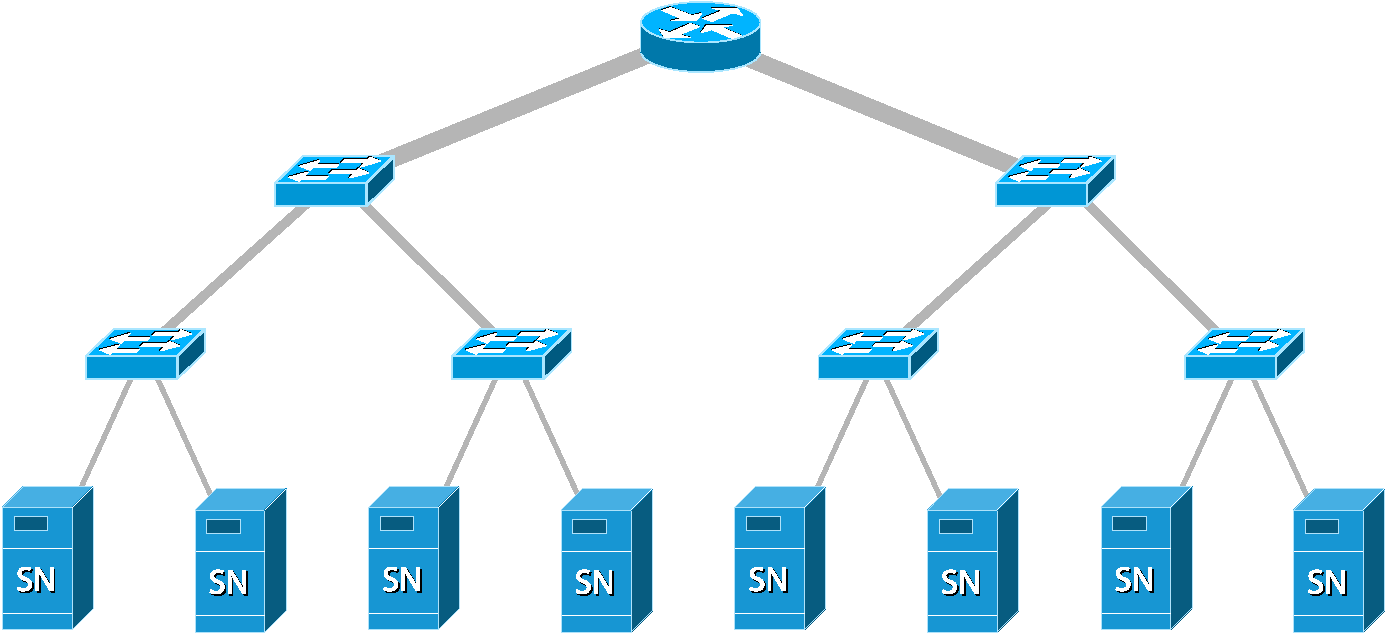
\includegraphics[autoebb, width=180pt]{./img/hierarchy_topology.pdf}
    \caption{階層型ネットワークトポロジー}
    \ecaption{Hierarchical network topology}
    \label{fig:hierarchical}
    \end{center}
\end{figure}

\begin{figure}[h]
\begin{minipage}{0.5\hsize}
\begin{center}
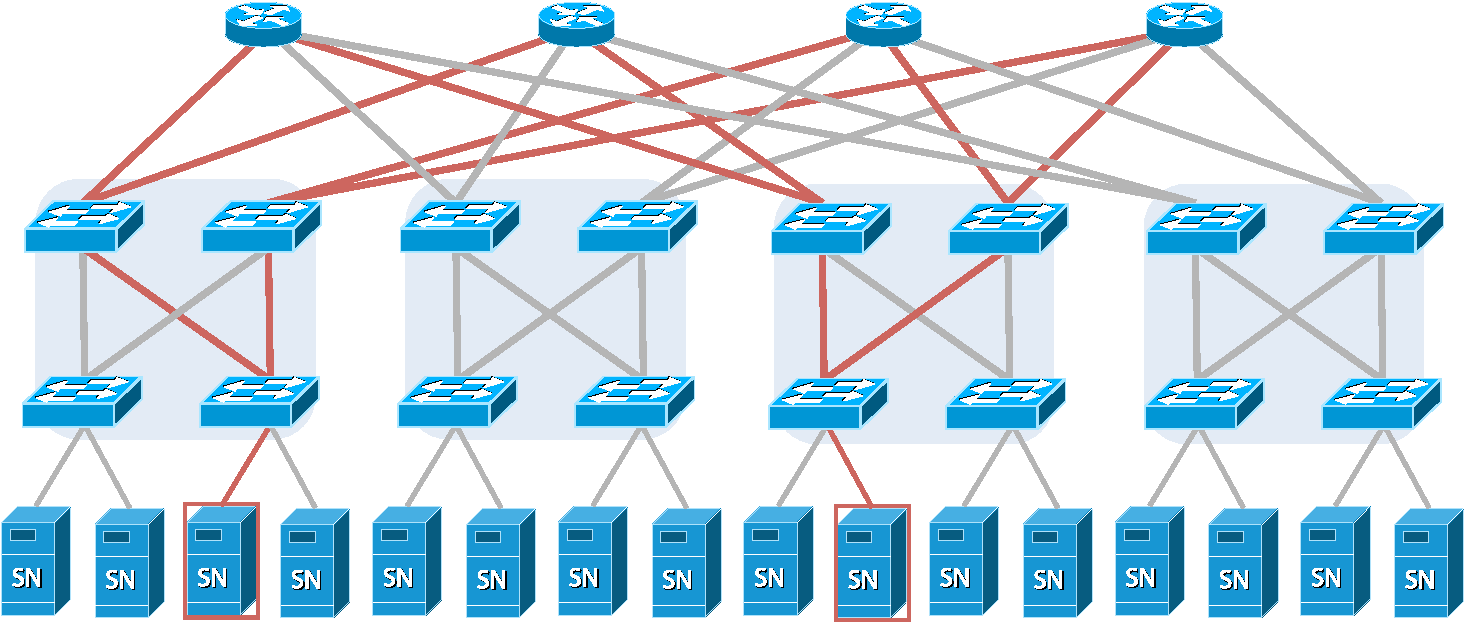
\includegraphics[autoebb, width=110pt]{./img/fattree_topology.pdf}
\end{center}
\caption{FatTreeトポロジー}
\ecaption{Fattree topology}
\label{fig:fattree}
\end{minipage}
\begin{minipage}{0.5\hsize}
\begin{center}
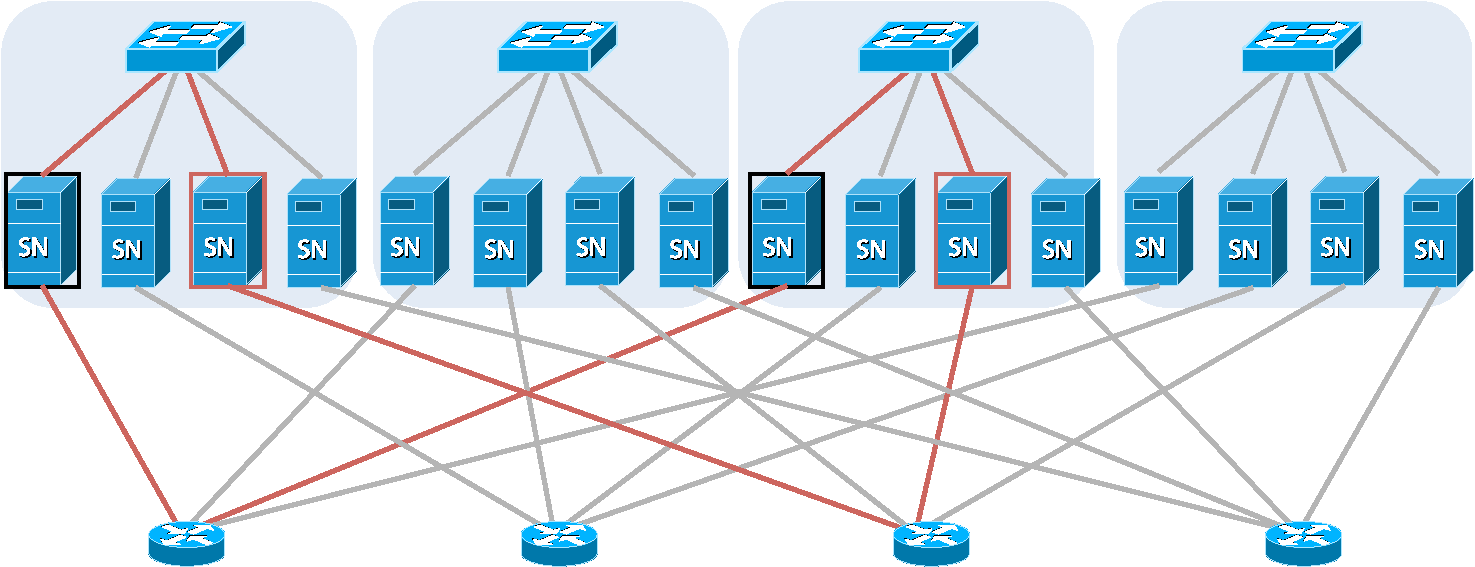
\includegraphics[autoebb, width=110pt]{./img/bcube.pdf}
\end{center}
\caption{BCubeトポロジー}
\ecaption{BCube topology}
\label{fig:bcube}
\end{minipage}
\end{figure}


\section{データセンターにおけるトラフィックシナリオ}
\label{sec:traffic_scenario}
本章では, データセンターにおけるトラフィックの特性について, 考察を行う.

大量の計算機資源を有効活用するためには, 分散処理フレームワークを用いる.
Hadoopが代表的なフレームワークとして使われており,
一般的に図\ref{fig:part_aggr}に示すようにpartition-aggregate構造をとる.
分散処理フレームワークでは, 多数の処理ノードと, 分散処理の制御をする管理ノードの二つのノードから構成されており, 管理ノードから, Queryが発行され, 分散処理がそれを受け取り,レスポンスを返す.
このとき, トラフィックパターンが  (1){\it Query traffic}, (2){\it Short message
traffic}, (3){\it Backgroung traffic}の3つに分類される~\cite{dctcp}.

{\bf Query traffic. }Query trafficとは, 大規模計算処理を分割して並列処理する際に,
aggregatorノードから処理ノードへ具体的な処理を割り当てるためのトラフィックである.
Query trafficの特徴は, 非常に小さいフローサイズ(2KB$\sim$20KB)で、処理全体のレイテンシに非常に強く影響を及ぼす事である.
また分散処理システムの構成上, Query trafficはms$\sim$µs単位でQueryが生成され,
バースト性を持つと言える~\cite{dctcp}.

{\bf Short message traffic. } Short message trafficとは,
処理ノードの動作を制御するためのトラフィックである.
Short message trafficの特徴は, フローサイズは50KB$\sim$1MBで, Query
trafficと同様に処理全体のレイテンシに影響を及ぼすという事である.
しかし, Querry trafficほどのフロー数は生成されず, 生成時間間隔も秒単位である.

{\bf Backgroung traffic. }Backgroung trafficは, Queryに対するレスポンスの精度を高める,
各処理ノードへ更新データを送信するトラフィックである.
Backgroung trafficの特徴は,フローサイズが1MB$\sim$50MBと大きいことにある.
さらに, その生成時間間隔は大きい.
また, Backgroung trafficでの更新データは, 処理精度の向上に寄与するが, 処理に必須ではないので,
処理全体のレイテンシにはつながらない.
また, Alizadehらは, 実際に利用されているデータセンターのトラフィックを分析した結果, Background trafficが発生する数は少ないが,
全体の通信量の大部分がBackgroung trafficによって占められていると報告しており,
経路全体へ影響を及ぼす可能性があることを示している~\cite{traffic}.

つまり, データセンターネットワークのトラフィックのうち, 分散処理開始時に生成されるQuery trafficが遅延すると,
処理全体に対し遅延を引き起こすので, Query trafficのフロー完結時間は極めて重要なメトリックである.

\begin{figure}[h]
    \begin{center}
    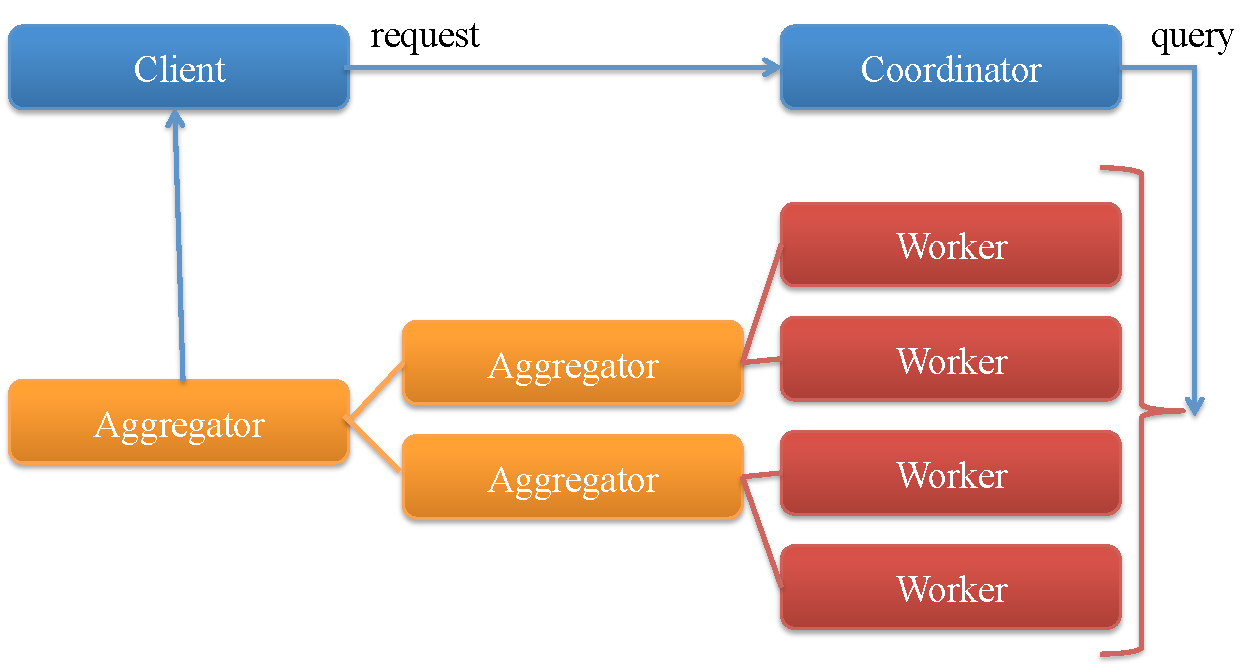
\includegraphics[autoebb, width=180pt]{./img/part_aggr.pdf}
    \caption{分散処理でのpartition-aggregate計算モデル}
    \ecaption{Partition-aggregate model on distribution system}
    \label{fig:part_aggr}
    \end{center}
\end{figure}


\section{再現実験と考察}
\label{sec:reproduction}
この章では,
Raiciuらによって示したFatTree-MPTCPネットワークモデルでのフローサイズの小さいトラフィックに対する性能評価シミュレーションを再現し,
解析を行った結果を示す.

\subsection{シミュレーション概要}
Raiciuらは~\cite{improving}において, 各プロトコルがフローサイズの小さなトラフィックに対して及ぼす影響の評価を行っており,
フローサイズの小さいトラフィックに関しては, MPTCPによりフロー完結時間を遅延させることを示した.
そのときのシミュレーション環境は, 以下の通りである.
ネットワークトポロジーには, 4:1にオーバーサブスクリプションされたFatTreeを用いている.
ベンチマークトラフィックについては, host-to-hostの1対1通信を用いている.
全てのhost-to-host通信のうち, 33\%をTCPまたはMPTCPにより継続してデータ転送(Back-ground traffic)を行う.
残りのhostを使って, TCPによる70Kbyteのデータ転送をを毎200[ms]のポアソン生起させ, 転送完了までにがかかった時間を計測している.

\subsection{再現シミュレーション実験環境}
今回, 再現実験にはns-3 Direct Code Execution~\cite{ns3}を用い, MPTCPは, Linux
カーネルソースを用いた~\cite{mptcp_linux}.
図\ref{fig:fattree_rep}に, シミュレーションで用いたFatTree(k=2)トポロジーを示す.
図\ref{fig:fattree_rep}の物理パスでは, 一つのサブフローが1本の物理パスを占有するように, 設計した.
すなわち, 4つのサブフローを使う場合, ホストには4本のインターフェースに対しそれぞれ4つIPアドレスが割り当てられる.
また, host-edge部分には, IPアドレスの数だけインターフェースを用意し, aggr-edge部分も, それに従いインターフェースを設置する.
さらに, ルーティングに関しては, core1$\sim$core4に分散するようにルーティングテーブルを設定した.
Singlepath-TCPを用いる場合は, Pod番号ごとに中継するcoreが分散するように設定した.

表\ref{table:testbed}に再現シミュレーション環境に対する各パラメータをまとめる.
\begin{table}[h]
\begin{center}
\begin{tabular}{c|c}
\hline
環境パラメータ & 値 \\ \hline \hline
ノード数 & 16 \\
Multipath TCP & v0.86 \\
帯域-core-aggr & 400Mbps \\
帯域-aggr-edge & 200Mbps \\
帯域-edge-host & 100Mbps \\
RTT & 0.5ms\\
バッファ & 100KB \\
\hline
\end{tabular}
\caption{ネットワークシミュレーション環境}
\ecaption{Testbed on network simulation}
\label{table:testbed}
\end{center}
\end{table}

\begin{figure}[h]
    \begin{center}
    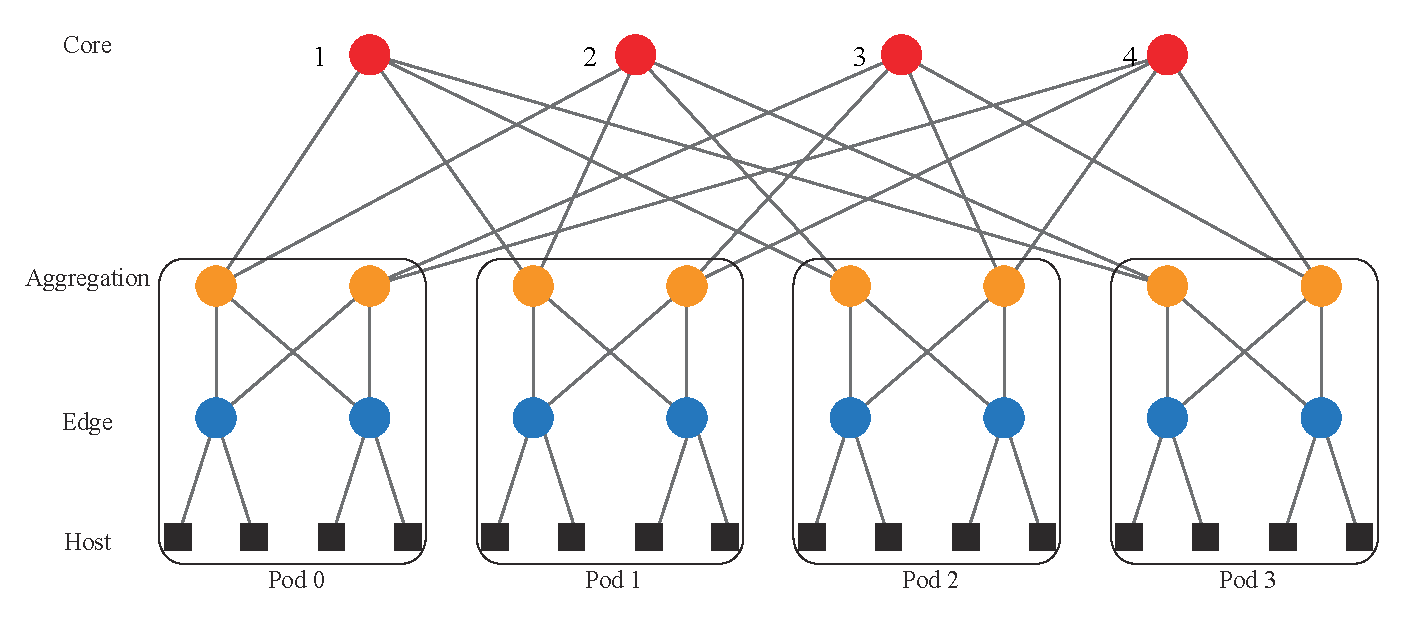
\includegraphics[autoebb, width=200pt]{./img/fattree_rep.pdf}
    \caption{再現シミュレーション環境でのネットワークトポロジー}
    \ecaption{Network topology on reproducing simulation}
    \label{fig:fattree_rep}
    \end{center}
\end{figure}

\subsubsection{設定パラメータに対する有効性の検証}
伝搬遅延についてはRTT(Round Trip Time)として, 0.5[ms]に設定した.
これは, 一般的なデータセンター内のRTTが0.5[ms]であるからである~\cite{rtt}.

ウィンドウサイズについては, 以下の帯域幅遅延積(BDP)の式から, 400Mbpsを最大限利用できるだけの値を設定した.
\begin{eqnarray}
BDP[{\rm byte}] = 帯域幅[{\rm bps}] \times RTT \div 8
\label{cong}
\end{eqnarray}

しかし, 各帯域については, 16のノードを使って輻輳を引き起こす現象を再現するために, 実際のデータセンターのような広帯域のネットワークと比べ,
狭い帯域を設定した

\subsection{再現結果}
図\ref{fig:short_flow_rep}, 表\ref{table:short_flow_rep},
表\ref{table:percentile}に, 上記の実験環境で再現した結果を示す.

再現結果から, フローの様子を完結時間別に4パターンに分類することができることが分かった.
表\ref{table:flow_pattern}にそのフローパターンの定義を示す.

\begin{figure}[h]
    \begin{center}
    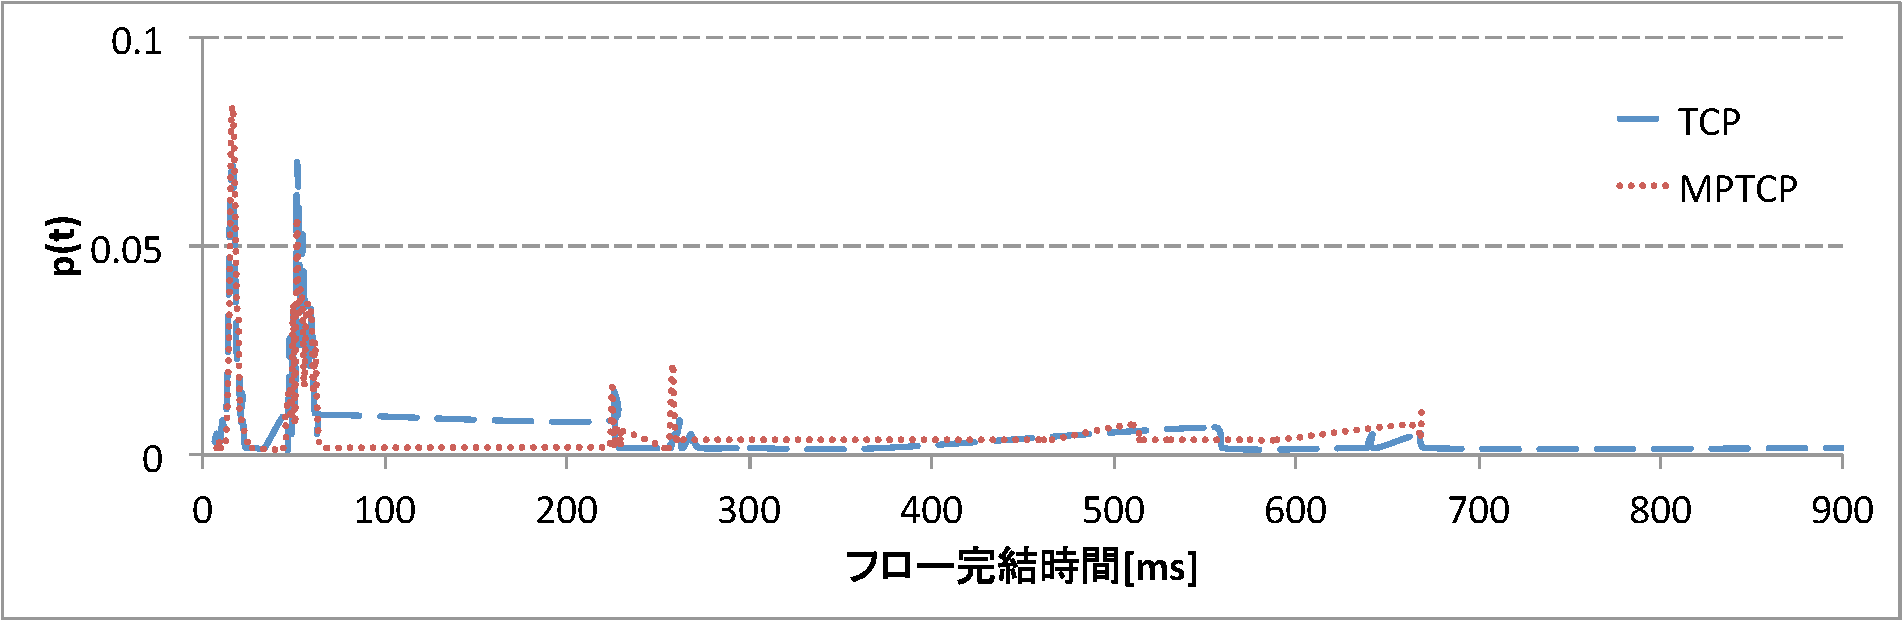
\includegraphics[autoebb, width=245pt]{./img/flow_comp.pdf}
    \caption{再現実験結果}
    \ecaption{The result of the reproduction experiment}
    \label{fig:short_flow_rep}
    \end{center}
\end{figure}

\begin{table}[h]
\begin{center}
\begin{tabular}{c|c|c}
\hline
プロトコル & 平均フロー完結時間[ms] & 標準偏差[ms]\\ \hline \hline
Single-Path TCP & 78.4 & 122.5 \\
MPTCP & 91 & 140.6\\
\hline
\end{tabular}
\caption{再現実験-平均フロー完結時間, 標準偏差}
\ecaption{Average flow completion time and stdev on reproduction experiment}
\label{table:short_flow_rep}
\end{center}
\end{table}

\begin{table}[h]
\begin{center}
\begin{tabular}{c|c}
\hline
プロトコル & $95^{th}$パーセンタイルフロー完結時間[ms] \\ \hline \hline
TCP & 266.7 \\
MPTCP & 510.5 \\
\hline
\end{tabular}
\caption{95パーセンタイルフロー完結時間}
\ecaption{$95^{th}$percentile completion times}
\label{table:percentile}
\end{center}
\end{table}

\begin{table}[h]
\begin{center}
\begin{tabular}{c|c|c}
\hline
フローパターン & 完結時間[ms] & パケットロスの有無 \\ \hline \hline
Full window & $\sim$30 & なし\\
Intensive flow & $\sim$60 & なし\\
Delay with loss & 200$\sim$300 & あり\\
Extreme delay & 300$\sim$ & あり\\
\end{tabular}
\caption{完結時間別のフローパターン}
\ecaption{Flow pattern classified by completion time}
\label{table:flow_pattern}
\end{center}
\end{table}


\subsection{考察}
表\ref{table:flow_pattern}に示した各フローパターンについて, それぞれの特性を分析する.

\subsubsection{パケットロスが発生しないフローパターン}
図\ref{fig:full_intensive}にFull windowとIntensive flowのデータ転送の様子を示す.
いずれのフローパターンもデータ転送中にパケットロスは発生しなかった.

Full windowでは, TCPコネクション確立後, サーバーがすぐに最大ウィンドウサイズ分だけパケットを送り,
クライアントからのACKが返ってくると, 随時次のパケットを送っていた.
これは, 経路に輻輳がなく, 多くのウィンドウを利用できたということであり, 30[ms]以下でデータ転送を完了した.

一方, Intensive flowでは, サーバーが最大ウィンドウサイズ分に満たない量のパケットを送り,
クライアントからまとめて送られてくるACKを受け取った後, 集約してパケットを送っていた.
その結果, コネクションの切断時に, Full windowと比較して遅延を引き起こし60[ms]程度転送時間がかかった.


\subsubsection{パケットロスが生じたフローパターン}
図\ref{fig:delay_loss}にDelay with lossとExtreme delayのデータ転送の様子を示す.
いずれのフローパターンもデータ転送中にパケットロスが発生し, 再送処理, 重複ACK確認応答を行った.
パケットロスが起きた原因は, 短時間にフローサイズの小さいトラフィックが中継ルータを集中したためである.
実際, 200[ms]のポアソン生起のうち, 数十ms単位でトラフィックが発生したとき, 中継ルータにおいてパケットロスが生じた.

Delay with lossでは, TCPコネクション確立後に数パケットのデータ転送を行い, パケットロスによるタイムアウトを生じた.
その後, 再送処理を経て, Ethernetフレームが最大1518[byte]でパケットを伝送した.

一方, Extreme delayでは, TCPコネクション確立直後にパケットロスによるタイムアウトを生じた.
その後も, パケットロスは生じないものの, 400[ms]頃まで遅延が生じていた.
また, 図\ref{fig:delay_loss}における二つのフローの傾きは, Ethernetフレームが586[byte]に設定され,
転送速度が上がらなかったことを表している.
これは, 中継するルータにおいてQoE制御による帯域制限が発生したことを示している.
実際, 同時刻に流れていたBack-ground trafficのスループットには変化がなく, QoE制御のrate controlによりBack-ground
trafficのデータ転送が優先されていた.

\begin{figure}[!h]
    \begin{center}
    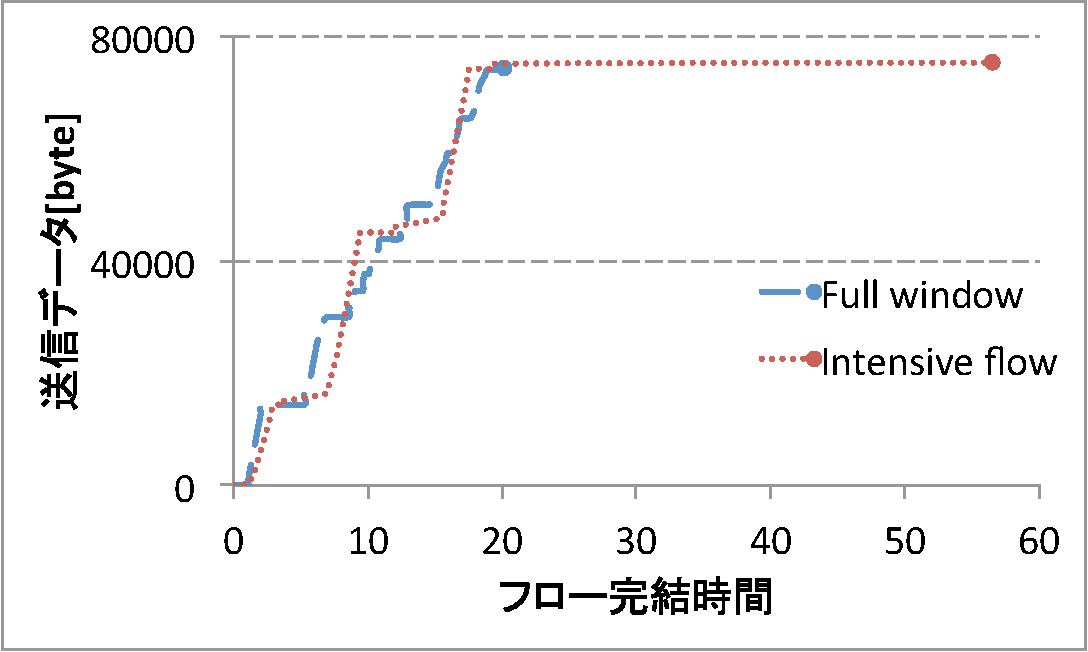
\includegraphics[autoebb, width=180pt]{./img/full_intensive.pdf}
    \caption{Full windowとIntensive flowの比較}
    \ecaption{Comparison between Full window and Intensive flow}
    \label{fig:full_intensive}
    \end{center}
\end{figure}

\begin{figure}[h]
    \begin{center}
    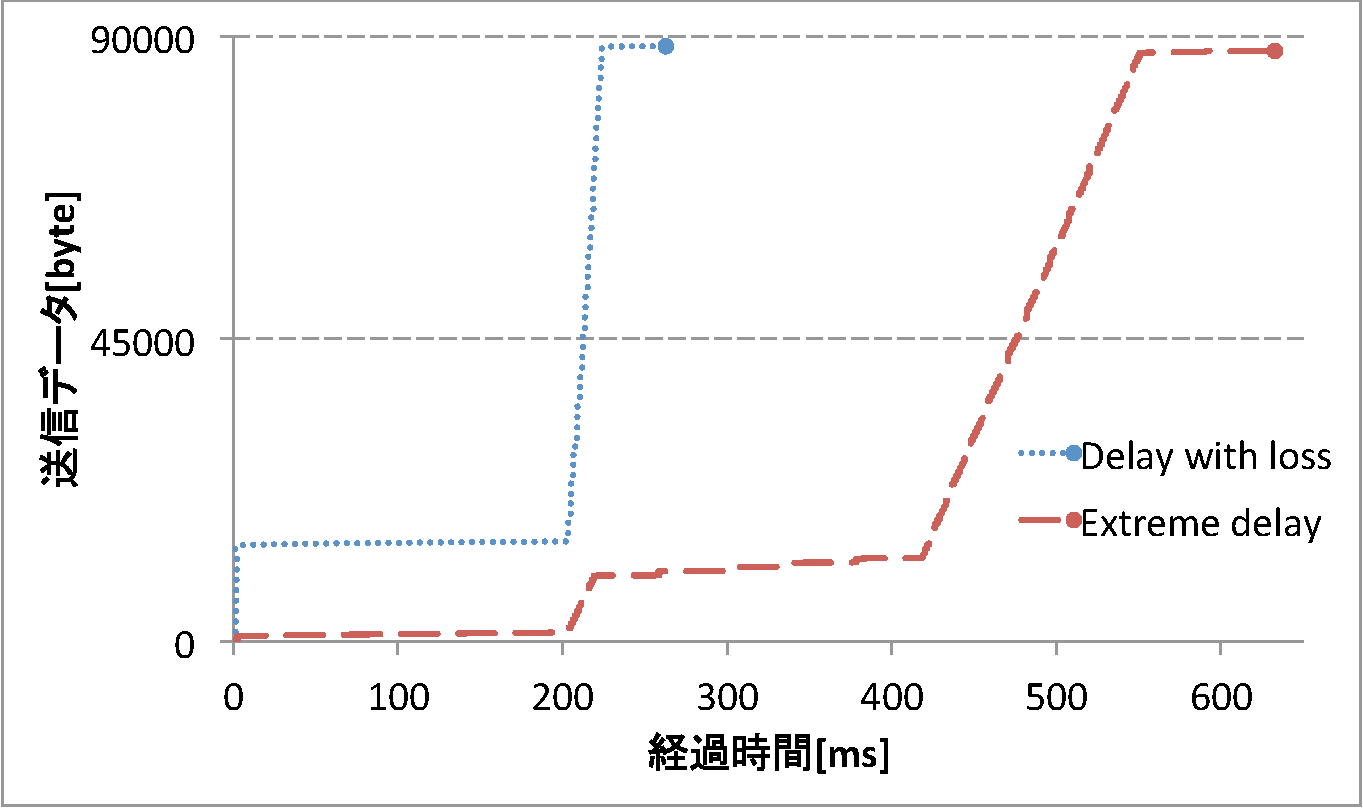
\includegraphics[autoebb, width=180pt]{./img/loss.pdf}
    \caption{Delay with lossとExtreme delayの比較}
    \ecaption{Comparison between Extreme delay and Extreme delay}
    \label{fig:delay_loss}
    \end{center}
\end{figure}

\subsubsection{TCP v.s. MPTCP}
今回の再現実験において, TCPとMPTCPでフロー完結時間に差を生じた要因は, パケットロスが発生する割合にある.

図\ref{fig:delay_loss}, 表\ref{table:percentile}に再現実験でのフロー完結時間ごとの累積確率分布を示す.
パケットロスを生じないフローに関しては, 両者に性能差を感じなかったが, この図から, MPTCPを用いた方が,
パケットロスを引き起こし遅延を生じさせる割合が大きいということが分かる.

このようにMPTCPが帯域を大きく占有することにより他のトラフィックを圧迫することは, MPTCPのCongestion
controlによるものだと考えられる.
混雑のない経路でデータ転送する場合, MPTCPでは積極的にウィンドウサイズを増やそうとするため, 他のフローに対し遅延を引き起こす.


\begin{figure}[h]
    \begin{center}
    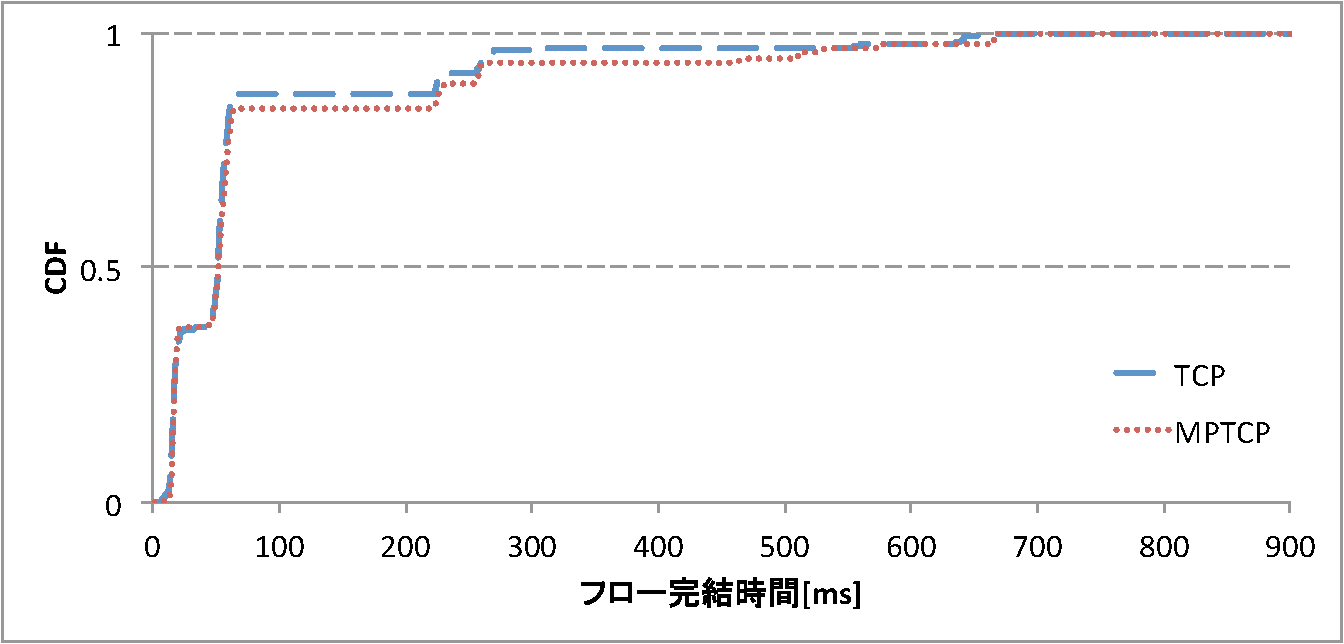
\includegraphics[autoebb, width=180pt]{./img/cdf_rep.pdf}
    \caption{再現実験でのフロー完結時間の累積確率分布}
    \ecaption{CDF of flow completion time on reproduction experiment}
    \label{fig:delay_loss}
    \end{center}
\end{figure}

\section{評価実験と考察}
\label{sec:evaluation}
この章では, MPTCPデータセンターネットワークに対して実際のデータセンター環境を想定したシミュレーション実験を行い, その結果について考察する.

\subsection{想定環境}
今回, データセンター上でpartition-aggregateモデルに従う分散処理を想定する.
ネットワークトポロジーについては, 前章のFatTreeトポロジーを用い, 一つのPodが管理ノード群として他Podの12ノードに対し,
処理を指示することを想定する.
またベンチマークトラフィックについては, \ref{sec:traffic_scenario}章で述べたような, 3つのトラフィックパターンが混在するとし,
それぞれについて評価・考察を行う.
メトリックとして表\ref{metric}を考える.
\begin{table}[h]
\begin{center}
\begin{tabular}{c|c}
\hline
トラフィックパターン & メトリック \\ \hline \hline
Query traffic & フロー完結時間[sec] \\
Short message traffic & フロー完結時間[sec] \\
Background traffic & スループット[bps] \\
\hline
\end{tabular}
\caption{トラフィックパターンごとのメトリック}
\ecaption{Metric of each traffic patern}
\label{metric}
\end{center}
\end{table}

\subsection{シミュレーション結果}

\subsubsection{Query traffic}
Query trafficに対する評価として, フローサイズは1[KB]$\sim$16[KB]とした,
12の処理ノードへ平均200[ms]のポアソン生起でトラフィックを発生させ, フロー完結時間を測定した.
また, Query trafficのみ発生させた場合と, 50\%の処理ノードに対し継続的にデータを送信するトラフィックを, Background
trafficとして同時に発生させた場合の2パターンについて評価を行った.
その結果を, 図\ref{fig:pure_query}, \ref{fig:mix_query}に示す.
なお, エラーバーとして99\%信頼区間を採用した.

この結果から, MPTCPはQuery trafficに対し, 直接性能に影響を及ぼさず, Background
Trafficによる影響が性能差を生じさせたことが分かる.
これは, やはりMPTCPがTCPよりも帯域を大きく占有した影響を受けたと考えられる.

\begin{figure}[h]
    \begin{center}
    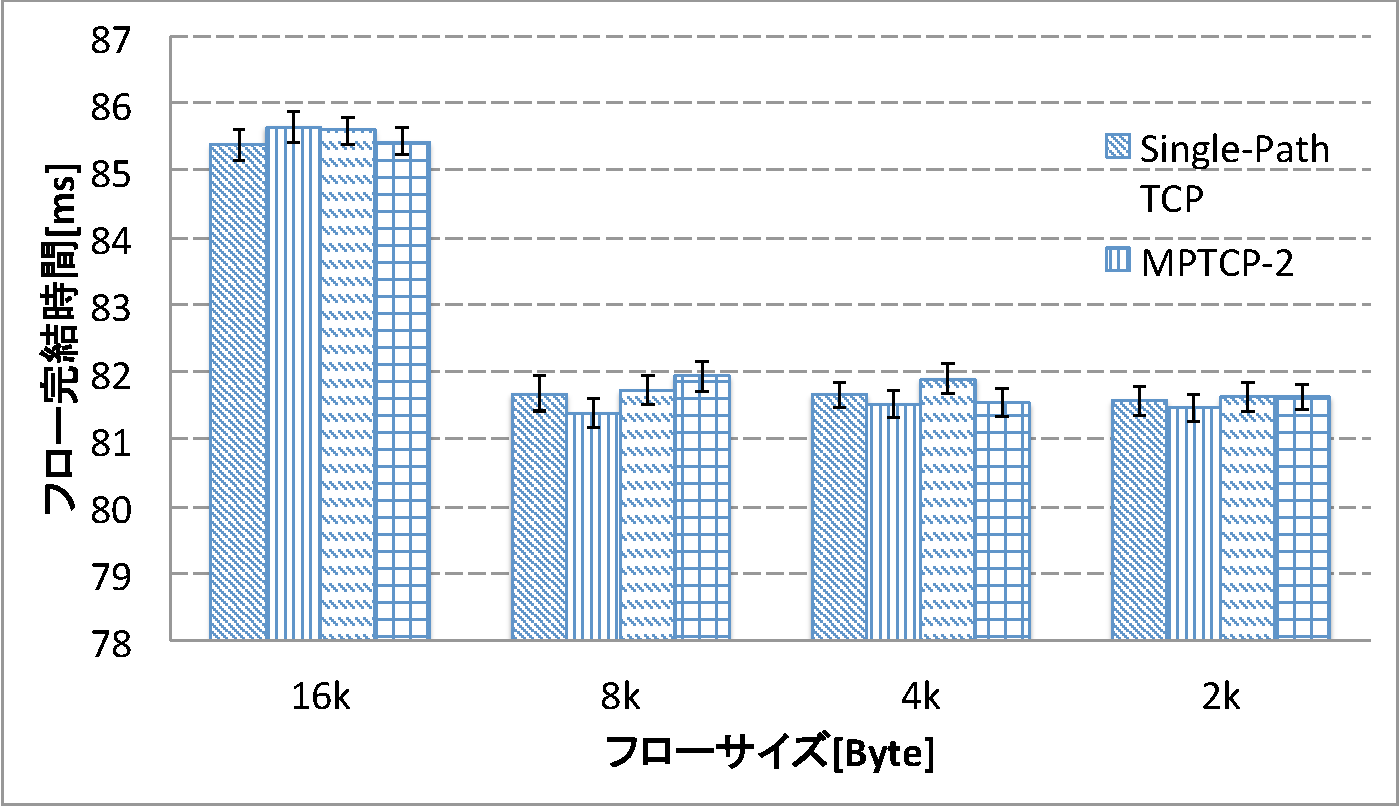
\includegraphics[autoebb, width=180pt]{./img/pure_query.pdf}
    \caption{Query trafficフロー完結時間(Background trafficなし)}
    \ecaption{Flow completion time  of Query traffic with Background traffic}
    \label{fig:pure_query}
    \end{center}
\end{figure}

\begin{figure}[h]
    \begin{center}
    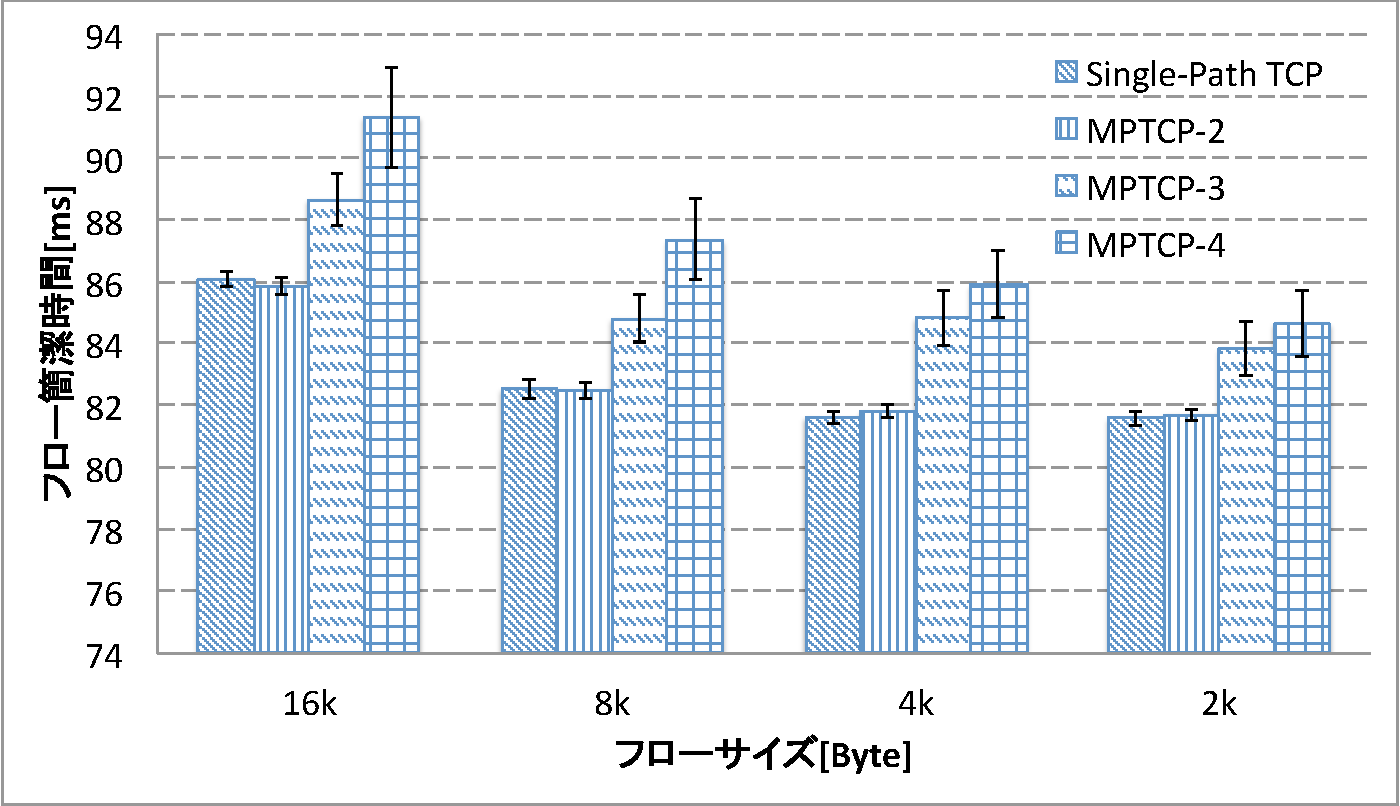
\includegraphics[autoebb, width=180pt]{./img/mix_query.pdf}
    \caption{Query trafficフロー完結時間(Background trafficあり)}
    \ecaption{Flow completion time  of Query traffic with Background traffic}
    \label{fig:mix_query}
    \end{center}
\end{figure}
\hspace{1cm}
\subsubsection{Short message traffic}
Short message trafficに対する評価として, フローサイズは50[KB]$\sim$1[MB]とした.
50\%の処理ノードに対し継続的にデータを送信するトラフィックを, Background trafficとして同時に発生させた状態で,
同時に12の処理ノードへ平均500[ms]のポアソン生起でトラフィックを発生させ, フロー完結時間を測定した.
その結果を, 図\ref{fig:short_query}に示す.

この結果から, MPTCPはShort message trafficに対し, フロー完結時間を短縮させたことが分かる.
これは, 先ほどのQuery trafficよりも大きなサイズのフローを流したので, MPTCPにより複数経路を利用し, TCPよりも短縮したことが考えられる.
実際, フローサイズが小さいと, MPTCPとTCP間でフロー完結時間の差が小さくなっている.

\begin{figure}[h]
    \begin{center}
    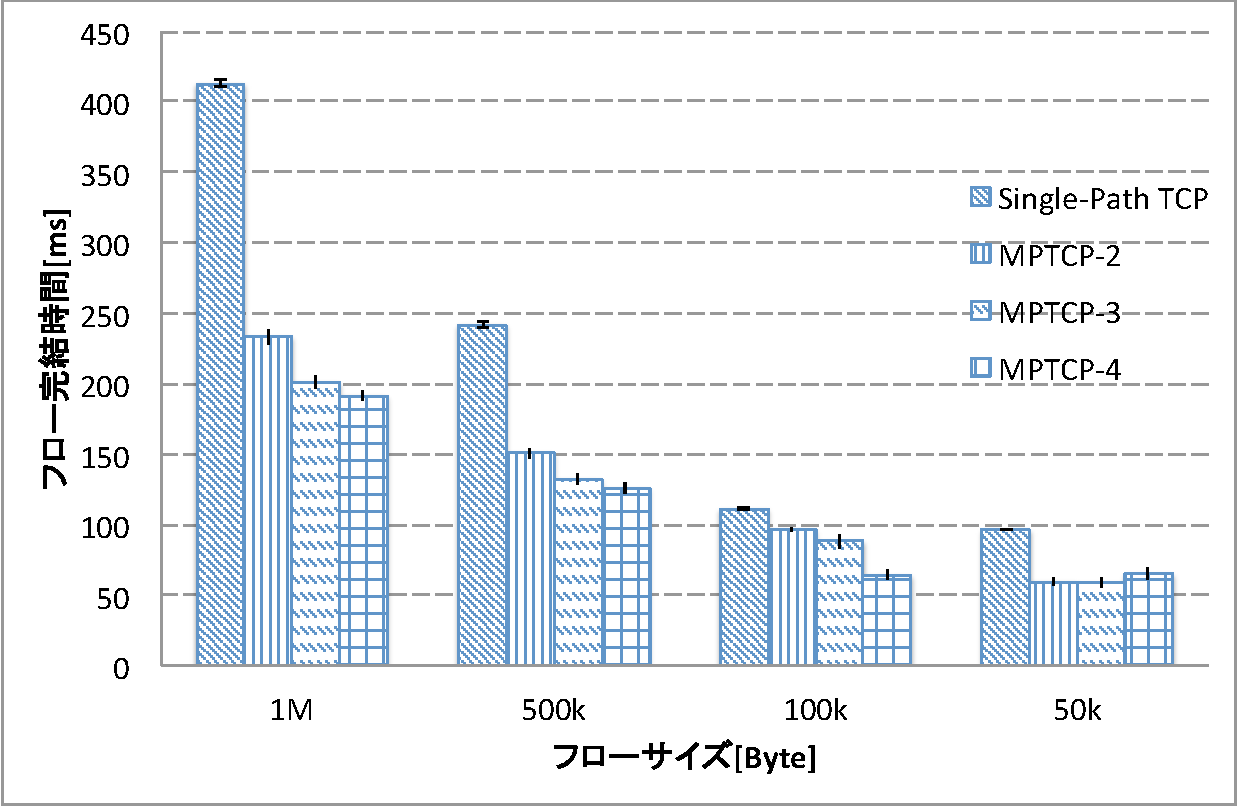
\includegraphics[autoebb, width=180pt]{./img/mix_short.pdf}
    \caption{Short message trafficフロー完結時間(Background trafficあり)}
    \ecaption{Flow completion time  of Short message traffic with Background
    traffic}
    \label{fig:short_query}
    \end{center}
\end{figure}


\subsubsection{Background traffic}
Background
trafficに対する評価として全12の処理ノードへ平均500[ms]のポアソン生起でフローサイズ1[KB]$\sim$1[MB]のトラフィックを同時に発生させた状態で,
同時に12の処理ノードへ平均500[ms]のポアソン生起でトラフィックを発生させ, 各経路のスループットを計測した.
その結果を図\ref{fig:background}に示す.

この結果から, MPTCPはBackground trafficに対し, TCPよりも性能向上が見られることが分かる.
これは, MPTCPのロードバランスと複数経路を使って並行的にデータを送信したことによるものである.

\begin{figure}[h]
    \begin{center}
    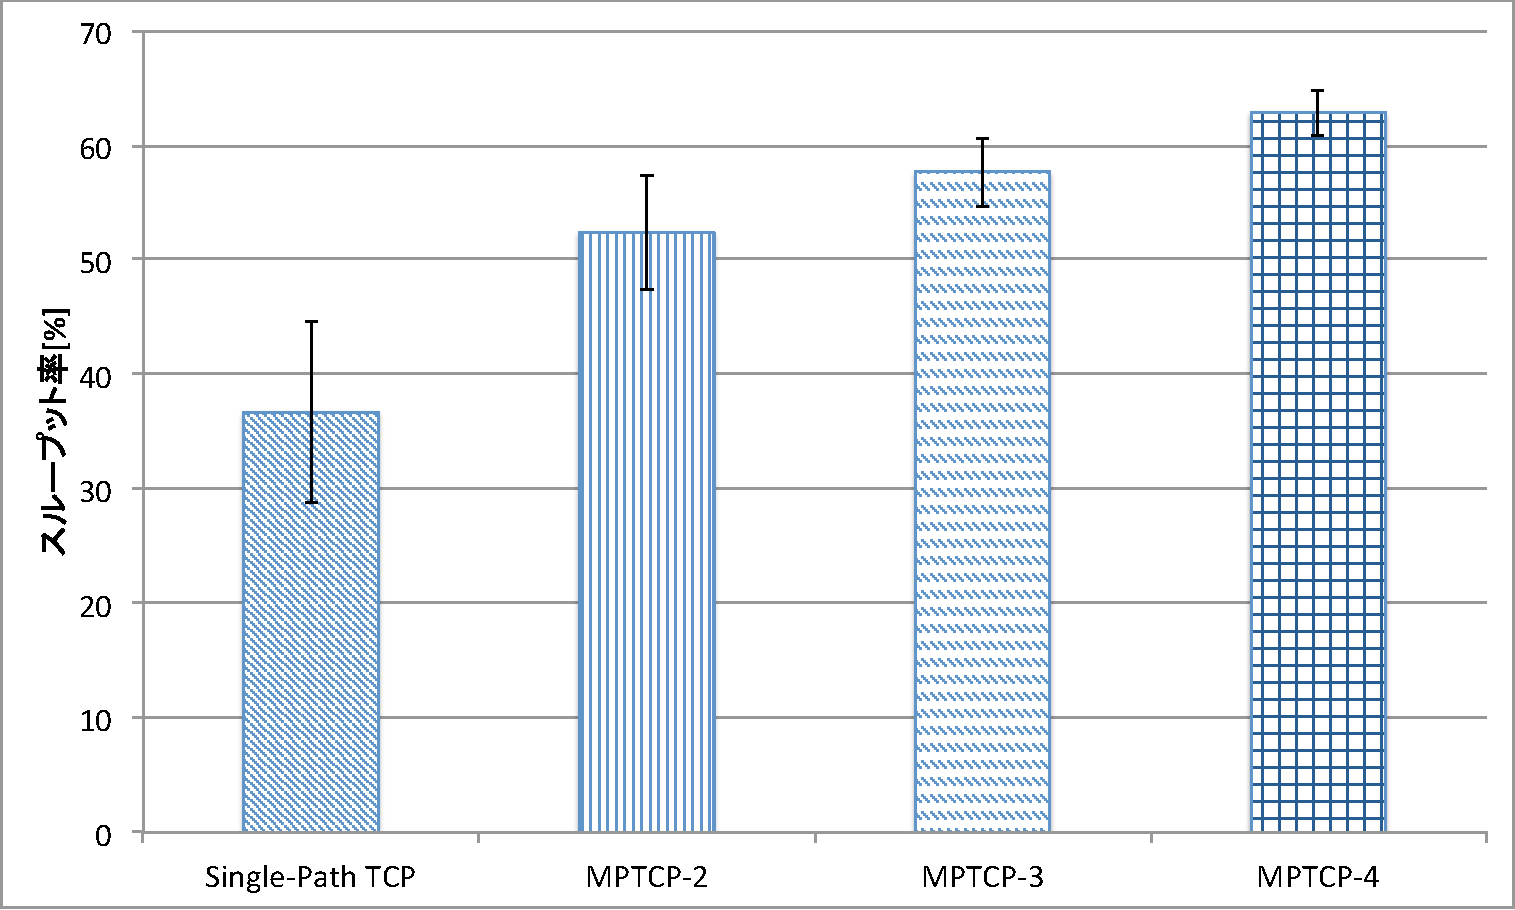
\includegraphics[autoebb, width=180pt]{./img/back.pdf}
    \caption{Background trafficスループット}
    \ecaption{Throughput of background traffic}
    \label{fig:background}
    \end{center}
\end{figure}
\hspace{1cm}

\section{あとがき}
\label{sec:conclude}
本論文では, MPTCPのフローサイズの小さいトラフィックに対しては,
従来のTCPよりもデータ転送に時間がかかるという報告~\cite{improving}を再現し, その原因を分析した.
その結果, 4つのフローパターンに分類することができ, そのうち, パケットロスが生じるフローがデータ転送時間に影響を及ぼすということを示した.
特に, MPTCPではフローサイズの大きいトラフィックが小さいトラフィックを圧迫し, パケットロスを引き起こす割合が高く,
その輻輳制御の公平性に問題が有るということを示した.
このことから, MPTCPが帯域を占有する問題を解消できれば, 従来のTCPを用いたデータセンターモデルよりも多様なトラフィックに対し性能の向上を期待される.

今後はOpenFlowによるトラフィック監視により, パケット衝突を引き起こさないロードバランスにより,
フローサイズによらずデータ転送高速化技術について検証していく予定である.

%\bibliographystyle{sieicej}
%\bibliography{myrefs}
\begin{thebibliography}{99}% 文献数が10未満の時 {9}
\bibitem{IBM_rep}{日本アイ・ビー・エム株式会社「IBM 第1章
大容量データのバックアップ」\url{http://www-06.ibm.com/systems/jp/storage/column/backup/01.html}}
\bibitem{amazon}{Jim Liddle. Amazon found every 100ms of latency cost them 1\%
in sales. , August 2008.
\url{http://blog.gigaspaces.com/amazon-found-every-100ms-of-latency-cost-them-1-in-sales/}}
\bibitem{presto}{Facebook「Presto: Interacting with petabytes of data at
Facebook」\url{https://www.facebook.com/notes/facebook-engineering/presto-interacting-with-petabytes-of-data-at-facebook/10151786197628920}}
\bibitem{mapreduce}{Dean, Jeffrey, and Sanjay Ghemawat. "MapReduce: simplified
data processing on large clusters." Communications of the ACM 51.1 (2008): 107-113.}
\bibitem{dryad}{Isard, Michael, et al. "Dryad: distributed data-parallel
programs from sequential building blocks." ACM SIGOPS Operating Systems Review 41.3 (2007): 59-72.}
\bibitem{fattree}{Al-Fares, Mohammad, Alexander Loukissas, and Amin Vahdat. "A
scalable, commodity data center network architecture." ACM SIGCOMM Computer Communication Review. Vol. 38. No. 4. ACM, 2008.}
\bibitem{bcube}{Guo, Chuanxiong, et al. "BCube: a high performance,
server-centric network architecture for modular data centers." ACM SIGCOMM Computer Communication Review 39.4 (2009): 63-74.}
\bibitem{vl2}{Greenberg, Albert, et al. "VL2: a scalable and flexible data
center network." ACM SIGCOMM Computer Communication Review. Vol. 39. No. 4. ACM, 2009.}
\bibitem{dctcp}{Alizadeh, Mohammad, et al. "Data center tcp (dctcp)." ACM SIGCOMM Computer Communication Review 40.4 (2010): 63-74.}
\bibitem{improving}{Raiciu, Costin, et al. "Improving datacenter performance and
robustness with multipath TCP." ACM SIGCOMM Computer Communication Review. Vol. 41. No. 4. ACM, 2011.}
\bibitem{detail}{Zats, David, et al. "DeTail: Reducing the flow completion time
tail in datacenter networks." ACM SIGCOMM Computer Communication Review 42.4 (2012): 139-150.}
\bibitem{click}{Kohler, Eddie, et al. "The Click modular router." ACM
Transactions on Computer Systems (TOCS) 18.3 (2000): 263-297.}
\bibitem{mptcp}{Ford, Alan, et al. TCP Extensions for Multipath Operation with
Multiple Addresses: draft-ietf-mptcp-multiaddressed-03. No. Internet draft (draft-ietf-mptcp-multiaddressed-07). Roke Manor, 2011.}
\bibitem{cong}{Raiciu, C., M. Handley, and D. Wischik. "Coupled congestion
control for multipath transport protocols." draft-ietf-mptcp-congestion-01 (work in progress) (2011).}
\bibitem{ns3}{Inria「DCE - GETTING STARTED Direct Code Execution」
\url{http://www.nsnam.org/~thehajime/ns-3-dce-doc/getting-started.html}}
\bibitem{traffic}{Benson, Theophilus, Aditya Akella, and David A. Maltz.
"Network traffic characteristics of data centers in the wild." Proceedings of the 10th ACM SIGCOMM conference on Internet measurement. ACM, 2010.}
\bibitem{mptcp_linux}{ip networking lab「MultiPath TCP - Linux Kernel
implementation」\url{http://mptcp.info.ucl.ac.be/}}
\bibitem{rtt}{Vasudevan, Vijay, et al. "Safe and effective fine-grained TCP
retransmissions for datacenter communication." ACM SIGCOMM Computer Communication Review. Vol. 39. No. 4. ACM, 2009.}

\end{thebibliography}

\begin{biography}
\profile*{s}{藤居 翔吾}{平25 立命館大・工。電気電子卒. 同年東京大学大学院修士課程入学.
Multipath TCPを利用したデータセンターネットワーク等の研究に従事.
}
\profile*{m}{関谷 勇司}{}
\profile*{m}{田崎 創}{}
%\profile{会員種別}{名前}{紹介文}% 顔写真あり
%\profile*{会員種別}{名前}{紹介文}% 顔写真なし
\end{biography}

\end{document}